\documentclass[12pt, a4paper]{article}
\usepackage{triada}
\usepackage{subfigure}
\usepackage{float}

\graphicspath{{eps/}{png/}}
\begin{document}

\tableofcontents

\newpage

\section{Задание 1}
\subsection{Постановка}
\begin{enumerate}
\item На основе генератора схемы Бернулли построить датчик для биномиального и отрицательного биномиального 
распределений.
\item На выборке объема $5000$ проверить эмпирически закон больших чисел.
\item Произвести $N=1000$ испытаний бернулли с вероятностью $\frac 12$ и интерполировать траекторию процесса $Y(t_n)=\frac{S_n}{\sqrt{N}}$ ломаной на отрезке $\left[0,1\right]$. $t_n = n/N,\ \linebreak S_n = \sum\limits_1^n X_n,\ X_n\in\left\{0,1\right\}$
\end{enumerate}
\subsection{Теоретическая часть}
\subsubsection{Определения и свойства}
\begin{df}
Случайная величина $X$ имеет \textit{распределение Бернулли} с параметром $p$, если она принимает лишь два значения, обычно $0$ и $1$, причем \[ \P(X = 1) = p,\ \P(X = 0) = 1-p. \]
\end{df}
\begin{df}
\textit{Схема Бернулли} состоит в проведении $N$ экспериментов (\textit{испытаний}), результатом каждого из которых может быть удача с вероятностью $p$ либо неудача с вероятностью $q=1-p$.
\end{df}
\begin{df}
\textit{Биномиальное распределение} $\Bi(n,p)$ --- распределение числа успехов в схеме Бернулли с $n$ экспериментами и вероятностью успеха $p$. 
\end{df}
Случайная величина $Y = \sum\limits_1^n X_i$, где $X_i$ имеют распределение бернулли с параметром $p$, имеет распределение $\Bi(n,p)$.
\begin{df}
\textit{Отрицательное биномиальное распределение} $\overline{\Bi}(r,p)$ --- распределение числа успехов в схеме Бернулли с вероятностью успеха $p$, предшествующих $r$-му неуспеху. 
\end{df}
И биномиальное, и отрицательное биномиальное распределение имеют свойство воспроизводимости по первому аргументу: если величины $X_i,\ i=\overline{1,k}$ имеют распределения $\Bi(n_i) \left( \overline{\Bi}(r_i,p) \right)$, то величина $Y = \sum\limits_1^k X_i$ имеет распределение $\Bi(n)  \left( \overline{\Bi}(r,p) \right)$, где $n=\sum\limits_{1}^{k}n_i \left( r = \sum\limits_{1}^{k}r_i \right)$.
\begin{df}
\textit{Геометрическим распределением} называется распределение $\overline{\Bi}(1,p)$.
\end{df}

Используя базовые факты комбинаторики, несложно найти функции вероятностей и математические ожидания для описанных распределений. Для биномиального распределения $P(X = k) = C_n^k p^k(1-p)^{n-k}$ и $\E(X) = np$ , а для отрицательного биномиального $P(X = k) = C_{k+r-1}^{k}p^r(1-p)^k$ и $\E(X)=\frac{n(1-p)}{p}$.

\subsubsection{Моделирование распределений}
Далее предполагается, что имеется возможность получать любое количество случайных чисел в отрезке $\left[0,1\right]$.

Принцип генерации бернуллиевских случайных величин таков: генерируется случайное число $x$ из отрезка $\left[0,1\right]$. Если $x < p$, то значение случайной величины полагается равным $1$, иначе равным $0$.

Для генерации биномиально распределенных случайных чисел используется свойство воспроизводимости. Известно, что $\Bi(1,p)$ --- распределение Бернулли с параметром $p$. Поэтому для получения величины, распределенной как $\Bi(n,p)$ генерируется $n$ бернуллиевскиx случайных величин с параметром $p$, и рассчитывается их сумма.

Геометрическое распределение генерируется по определению: генерируются случайные бернуллиевские величины, пока значение следующей не станет равным $1$. Количество сгенерированных случайных величин, уменьшенное на единицу, будет значением искомой случайной величины.

Отрицательное биномиальное распределение генерируется с использованием свойства воспроизводимости аналогично биномиальному.

\subsubsection{Закон больших чисел}
\begin{theorem}[Закон больших чисел]
Пусть $\left\{X_i\right\}_1^\infty$ --- последовательность одинаково распределенных попарно независимых случайных величин c математическим ожиданием $\mu$, заданных на одном вероятностном пространстве, тогда 
\[ \frac 1n \sum\limits_1^n X_i \to \mu \text{ почти всюду.}\]
\end{theorem}

\newpage

\subsection{Практическая часть}

\begin{figure}[H]
\subfigure[$n=10,\ p=0.5.$]{
\includegraphics[scale=0.45]{bin_n10_p05_sz1000.eps}
}
\subfigure[$n=10,\ p=0.3.$]{
\includegraphics[scale=0.45]{bin_n10_p03_sz1000.eps}
}
\begin{center}
\subfigure[$n=20,\ p=0.9.$]{
\includegraphics[scale=0.45]{bin_n20_p09_sz1000.eps}
}
\end{center}
\caption{Гистограммы значений $\Bi(n, p)$ на выборке размера $1000$. Черным обозначено смоделированное значение, синим --- теоретически рассчитанное.}
\end{figure}

\begin{figure}[H]
\subfigure[$r=1,\ p=0.4.$]{
\includegraphics[scale=0.45]{nbin_r1_p04_sz1000.eps}
}
\subfigure[$r=10,\ p=0.8.$]{
\includegraphics[scale=0.45]{nbin_r10_p08_sz1000.eps }
}
\begin{center}
\subfigure[$r=4,\ p=0.4.$]{
\includegraphics[scale=0.45]{nbin_r4_p04_sz1000.eps }
}
\end{center}
\caption{Гистограммы значений $\negBi(n, p)$ на выборке размера $5000$. Черным обозначено смоделированное значение, синим --- теоретически рассчитанное. Значения, вероятность которых меньше $\varepsilon=0.01$ опущены, чтобы не загромождать рисунок.}
\end{figure}

\begin{figure}[H]
\subfigure[$n=1,\ p=0.5$: ЗБЧ для частот.]{
\includegraphics[scale=0.45]{zbch_bi_1_05_5000.eps}
}
\subfigure[$n=5,\ p=0.7.$]{
\includegraphics[scale=0.45]{zbch_bi_5_07_5000.eps}
}
\caption{Синим цветом обозначен график эмпирического мат. ожидания, красным --- теоретического мат. ожидания для биномиальной величины. Размер выборки --- до 5000 элементов.}
\end{figure}

\begin{figure}[H]
\subfigure[$r=4,\ p=0.3,$ размер выборки $5000$]{
\includegraphics[scale=0.45]{zbch_nbi_4_03_5000.eps}
}
\subfigure[$r=4,\ p=0.3,$ размер выборки $50000$]{
\includegraphics[scale=0.45]{zbch_nbi_4_03_50000.eps}
}
\caption{Синим цветом обозначен график эмпирического мат. ожидания, красным --- теоретического мат. ожидания для отрицательной биномиальной величины. На выборке большей длины заметно лучшее выполнение ЗБЧ.}
\end{figure}

\begin{figure}[H]
\subfigure{
\includegraphics[scale=0.45]{orl1.eps}
}
\subfigure{
\includegraphics[scale=0.45]{orl2.eps}
}
\begin{center}
\subfigure{
\includegraphics[scale=0.45]{orl3.eps}
}
\end{center}
\caption{Возможные траектории игры в <<орлянку>>.}
\end{figure}

\newpage

\section{Задание 2}
\subsection{Постановка}
\begin{enumerate}
\item Реализовать генератор схемы Бернулли.
\item Построить датчик для сингулярного распределения, отвечающий канторовой функции распределения.
\item Для канторовых случайных величин проверить свойство симметричности относительно $\frac 12$ и самоподобия третей.
\item На построенном в п.\,2 датчике проверить эмпирически функцию распределения.
\end{enumerate}

\subsection{Теоретическая часть}
Генерация схемы бернулли была описана в первом задании.

\begin{df}
\textit{Канторово множество} $K$ --- множество чисел отрезка $[0,1]$, у которых в троичной записи нет единиц. 
\end{df}
Так как для всех чисел канторова множества (числа вида $0.\alpha_1\alpha_2\ldots,\ \alpha_i \in \left\{ 0,2\right\}$) Верно $\alpha_1\ne 1$, то канторово множество не содержит среднюю треть отрезка $[0,1]$. Так как $\alpha_2\ne 1$, то две оставшиеся трети не содержат средних третей, и так далее. Таков геометрический смысл канторова множества.

\begin{theorem}[Свойство симметричности]
Если $x\in K$, то и $1-x \in K$.
\end{theorem}
\begin{proof}
В троичной записи \[0.\beta_1\beta_2\ldots = 1-x = 0.(2) - 0.\alpha_1\alpha_2\ldots, \] 
поэтому \[\beta_i = 2 - \alpha_i,\ \alpha_i\in\left\{0,2\right\}\  i=1,\ldots.\]
Из этого следует, что в троичной записи числа $1-x$ нет единиц.
\end{proof}

\begin{theorem}[Свойство самоподобия]
Если $x\in K$, то и $\frac x3 \in K$.
\end{theorem}
\begin{proof}
В троичной записи \[\frac{x}{3} =0.0\alpha_1\alpha_2\ldots. \]
Из этого следует, что в троичной записи числа $\frac x3$ нет единиц.
\end{proof}	

Из курса функционального анализа \cite{Kolmogorov_Fomin} известно, что мера множества $K$ равна нулю.

Будем генерировать точки этого множества, используя определение: рассмотрим $N$ бернуллиевских независимых величин $X_i$ с параметром $\frac 12$, значением успеха $2$ и неуспеха $0$. Тогда случайное число из множества $K$ будет иметь следующий вид:
\[ Y = \sum\limits_1^n \frac{X_k}{3^k}. \]

Различные значения $N$ задают различную точность получения искомого случайного числа: $\frac{1}{3^{n}}$.

Имея большое количество случайных чисел $Y_i \in K$, можно найти \textit{эмпирическую функцию распределения}, соответствующую $K$ --- функцию, константную между двумя последовательными числами $Y_i$ и $Y_{i+1}$ и увеличивающуюся на $\Delta = \frac 1N$ в каждой точке $Y_i$.

\subsection{Практическая часть}
\begin{figure}[H]
\subfigure[$N=5.$]{
\includegraphics[scale=0.45]{kantor_5.eps}
}
\subfigure[$N=50.$]{
\includegraphics[scale=0.45]{kantor_50.eps}
}
\caption{Эмпирическая функция распределения. Выборка размером $5000$. Количество знаков после запятой $N$}
\end{figure}

\begin{figure}[H]
\subfigure[Симметричность.]{
\includegraphics[scale=0.45]{kantor_symm.eps}
}
\subfigure[Самоподобие.]{
\includegraphics[scale=0.45]{kantor_selfsim.eps}
}
\caption{Свойства полученной функции распределения.}
\end{figure}

\newpage

\section{Задание 3}
\subsection{Постановка}
\begin{enumerate}
\item Построить датчики экспоненциального и пуассоновского распределений.
\item Построить датчик нормального распределения методом получения пар случайных величин переходом к полярным координатам.
\item Построить датчик распределения $\chi^2$ с $n$ степенями свободы.
\end{enumerate}

\subsection{Теоретическая часть}
\subsubsection{Определения}
\begin{df}
\textit{Гамма-распределение} задается своей плотностью 
\[f(x) = x^{k-1} \frac{e^{-\frac{x}{\theta}}}{\Gamma(k)\theta^k}\cdot \left[ x \geqslant 0 \right].\]
\end{df}
Это распределение обладает свойством воспроизводимости по параметру $k$.
\begin{df}
\textit{Экспоненциальное распределение} задается своей плотностью 
\[f(x) = \lambda\exp{ \{-\lambda x\} }\cdot \left[ x \geqslant 0 \right],\ \lambda>0.\]
\end{df}
Для экспоненциально распределенной случайной величины $X$ математическое ожидание $\E X = \frac 1\lambda$.

Кроме того, экспоненциальное распределение --- частный случай Гамма-распределения с параметрами $k=1,\  \theta = \lambda^{-1}$.
\begin{df}
\textit{Пуассоновское распределение} --- дискретное распределение с функцией вероятности 
\[P(X = k) = \frac{\lambda^k}{k!}\exp{ \{ -\lambda\} },\ \lambda>0.\]
\end{df}
Для пуассоновской величины $X$ математическое ожидание $\E X = \lambda$.
\begin{df}
\textit{Нормальное распределение} --- распределение с плотностью
\[f(x) = \frac1{\sigma\sqrt{2\pi}}\; \exp\left\{ -\frac{\left(x-\mu\right)^2}{2\sigma^2} \right\}. \]
\end{df}
Математическое ожидание нормально распределенной величины равно $\mu$.

\begin{df}
\textit{Распределение $\chi^2$} с $n$ степенями свободы --- распределение суммы $n$ квдратов независимых случайных величин, нормально распределенных с параметрами $\mu = 0,\ \sigma^2 = 1$.
\end{df}

\subsubsection{Экспоненциальное и пуассоновское распределения}
Моделировать экспоненциальное распределение величины будем методом обратных функций, справедливость которого показана в \cite{Ivchenko_Medvedev}.
\begin{stm}
Если функция распределения $F(\cdot)$ некоторого распределения $\xi$ строго монотонна на всей числовой прямой, то существует обратная функция $F^{-1}(\cdot)$, причем если случайная величина $X$ равномерно распределена на отрезке $\left[0,1\right]$, то $F^{-1}(X)$ будет иметь функцию распределения $F(\cdot)$.
\end{stm}

Функция распределения для экспоненциальной случайной величины имеет вид \[ F(x) = 1 - \exp \{-\lambda x\}, \]
поэтому обратная к ней
\[F^{-1}(y) = -\frac{\ln \left(1 - y\right)}{\lambda}.\]

Таким образом, рассматривая равномерно распределенные на $[0,1]$ случайные величины и преобразуя их по полученной формуле, можно получать экспоненциально распределенные случайные величины.

Для моделирования пуассоновского распределения воспользуемся следующей теоремой.
\begin{theorem}
Случайная величина \[Y = \max\left\{n\colon \sum\limits_1^n X_i < 1 \right\},\]
где все $X_i$ попарно независимы и распределены экспоненциально с параметром $\lambda$, имеет пуассоновское распределение с таким же параметром.
\end{theorem}
\begin{proof}
Воспользуемся тем, что функция распреления гамма-распределения с натуральным параметром $k$, и параметром $\theta > 0$ имеет вид \[ F(x) = 1 - \sum\limits_0^{k-1} \frac{(\theta x)^i}{i!}\exp\{-\theta x\}  .\]
В таком случае, так как экспоненциальное распределение --- частный случай гамма-распределения, имеем
\begin{align*}
P(Y = n) &= P(X_1+\ldots+X_n < 1) - P(X_1+\ldots+X_{n+1} < 1) = \\ 
& = 1 - \sum\limits_0^{n-1} \frac{(\lambda x)^i}{i!}\exp\{-\lambda x\} -
    1 + \sum\limits_0^{n} \frac{(\lambda x)^i}{i!}\exp\{-\lambda x\} = \\
&   =\frac{\lambda^n}{n!}\exp \left\{ -\lambda \right\}.
\end{align*}
\end{proof}
Таким образом, для генерации пуассоновского распределения ищется значение:
\[\max\left\{n\colon -\frac 1\lambda\left(\ln(1-X_1)+\ldots+\ln(1-X_n)<1\right)\right\},\]
где все $X_i$ --- независимые, равномерно распределенные в $[0,1]$.
Заменим скобки $1-X_i$ на $X_i$, так как они распределены одинаково. Тогда полученное будет равносильно
\[ \max\left\{X_1\cdot\ldots\cdot X_n > \exp\left\{ -\lambda \right\}\right\}.\]

\subsubsection{Нормальное и $\chi^2$ распределения}
Для моделирования нормального распределения будем пользоваться методом, описанным и доказанным в \cite{Box_Muller}. Этот метод предполагает генерацию двух независимых стандартно нормально распределенных величин по двум равномерно распределенным в отрезке $[0,1]$ по формулам
\begin{align*}
Y_1 = \sqrt{ -2\ln X_1 } \sin(X_2\cdot 2\pi), \\
Y_2 = \sqrt{ -2\ln X_1 } \cos(X_2\cdot 2\pi).
\end{align*}

Для получения нормальных величин с произвольными параметрами $\mu,\ \sigma^2$ достаточно умножить значения реализаций стантартной нормальной величины на $\sigma$ и прибавить к ним $\mu$.

Генерация случайных величин с $\chi^2$ распределение проводится по определению, генерацией нескольких нормальных величин и их суммированием.

\subsection{Практическая часть}
\begin{figure}[H]
\subfigure[$\lambda = 1$.]{
\includegraphics[scale=0.45]{exp_1_1000.eps}
}
\subfigure[$\lambda = 5$.]{
\includegraphics[scale=0.45]{exp_5_1000.eps}
}
\caption{Экспоненциальное распределение. Красная кривая --- точные значения плотности. Выборка размера 1000.}
\end{figure}

\begin{figure}[H]
\subfigure[$\lambda = 1.5$.]{
\includegraphics[scale=0.45]{poiss_1d5_1000.eps}
}
\subfigure[$\lambda = 10$.]{
\includegraphics[scale=0.45]{poiss_10_1000.eps}
}
\caption{Пуассоновское распределение. Синие --- точные значения, черные --- смоделированные. Размер выборки 1000.}
\end{figure}

\begin{figure}[H]
\subfigure[$\mu = 0,\ \sigma^2 = 1$.]{
\includegraphics[scale=0.45]{norm_0_1.eps}
}
\subfigure[$\mu = -5,\ \sigma^2 = 5$.]{
\includegraphics[scale=0.45]{norm_m5_5.eps}
}
\caption{Нормальное распределение. Красная кривая --- точные значения плотности.}
\end{figure}

\begin{figure}[H]
\subfigure[$k=1$.]{
\includegraphics[scale=0.45]{chi2_1.eps}
}
\subfigure[$k = 5$.]{
\includegraphics[scale=0.45]{chi2_5.eps}
}
\caption{Распределение $\chi^2$. Красная кривая --- точные значения плотности.}
\end{figure}

\newpage

\section{Задание 4}
\subsection{Постановка}
\begin{enumerate}
\item Построить датчик распределения Коши.
\item Мажорируя плотность стандартного нормального распределения плотностью распределения Коши с параметрами сдвига $a$ и масштаба $b$, обеспечить максимальную эффективность метода фон Неймана моделирования нормального распределения.
\item Сравнить скорость моделирования в задании 3 и в задании 4.
\end{enumerate}

\subsection{Теоретическая часть}
\begin{df}
\textit{Распределение Коши} задается своей плотностью 
\[f(x) =\frac 1\pi \frac \gamma{\gamma^2 + (x-x_0)^2},\]
где $x_0$ --- параметр сдвига, а $\gamma > 0$ --- параметр масштаба.
\end{df}

Датчик распределения Коши строится методом обратных функций:
\[F(x) = \frac 1\pi \arctan\left(\frac{x-x_0}{\gamma}\right) + \frac 12 	\Rightarrow  F^{-1}(y) = x_0 + \gamma\tan\left(\frac 12 \pi (2y - 1)\right).\] 

По этой формуле можно получить из равномерно распределенной на $[0,1]$ величины $Y$ распределенную по Коши величину $X$.



\newpage

\addcontentsline{toc}{section}{Список литературы}
\bibliographystyle{sastyle}
\bibliography{library}

\end{document}